%!TEX root = main.tex
\section{Results and Discussion\label{sec:results}}

  \subsection{Experimental Setup}
    \par  A sub-sampled dataset was created from the full dataset to determine the efficacy of these algorithms on varying number of worker responses\techreport{, based on Table~\ref{batch_sample}}.
    \papertext{Every object was randomly sampled worker with replacement. For small worker samples, we average our results over larger number of batches than for large worker samples (which have lower variance, since the sample size is close to the original data size).} The number of workers plotted indicates the number of distinct worker segmentation used in the algorithm, note that in the clustered cases, the actual number of segmentation in the cluster may be less than what is cited in the sample. \techreport{In the subsequent section, we will refer to objects specific to a sample synonymously as objects.
      \begin{table}[ht]
      \centering
      \begin{tabular}{l|llllll}
      \# of workers & 5  & 10 & 15 & 20 & 25 & 30 \\ \hline
      \# of batches & 10 & 8  & 6  & 4  & 2  & 1 
      \end{tabular}
      \caption{Every object was randomly sampled worker with replacement. For small worker samples, we average our results over larger number of batches than for large worker samples (which have lower variance, since the sample size is close to the original data size).}
      \label{batch_sample}
      \end{table} }
  \subsection{Evaluation Metrics}
   \par Evaluation metrics used in our experiment measures how well the final segmentation (S) produced by these algorithms compare against ground truth (GT). The most common evaluation metric used in literature are area-based methods which take into account the intersection, $IA=area(S\cup GT)$, or union, $UA=area(S\cap GT)$, between the user and the ground truth segmentations. Specifically, we use
    $\text{Precision (P)} = \frac{IA(S)}{area(S)}$, 
    $\text{Recall (R)} = \frac{IA(S)}{area(GT)}$, and 
    $\text{Jaccard (J)} = \frac{UA(S)}{IA(S)}$
    metrics to evaluate our algorithms.
    % \\
    % $$\text{False Positive Rate (FPR)}= \frac{area(S)-IA}{area(GT)}$$\\
    % $$\text{False Negative Rate (FNR)}= \frac{area(GT)-IA}{(area(S)-IA)+(area(Image)-UA)}$$
%%%%%%%%%%%%%%%%%%%%%%%%%%%%%%%%%%%%%%%%%%%%%%%%%%%%%%%%%%%%%%%%%%%%%%%%%%%%%%%%%%%%%%%%%%%%%%%%%%%%%%%%%%%%%%%%%%%%%%%%%%%%%%%%%%%%%%%%%%
  \subsection{What is the difference in performance between retrieval and aggregation-based methods?}
    Figure~\ref{retreival_vs_aggregation} shows the comparisons between the best performing algorithm amongst aggregation-based (greedy, EM) and retrieval-based (num points) algorithms. The solid line in Figure~\ref{retreival_vs_aggregation} shows algorithms that does not make use of ground truth information as part of the inference, while the dotted line shows the corresponding algorithm that makes use of ground truth information. Amongst the algorithms that do not make use of ground truth information, the performance of the greedy and EM algorithms exceeds the best achievable through existing retrieval-based method via the \texttt{num points} scoring heuristic and the vision-based algorithms. 
    \par By examining the dotted ground-truth algorithms, we learn the best achievable aggregation-based algorithm performs far better than the best worker segmentation. This result demonstrates since aggregation-based methods performs inference at a finer \textit{tile} granularity, it is able to achieve better performance than compared to retrieval-methods.
    \begin{figure}[h!]
      \centering
      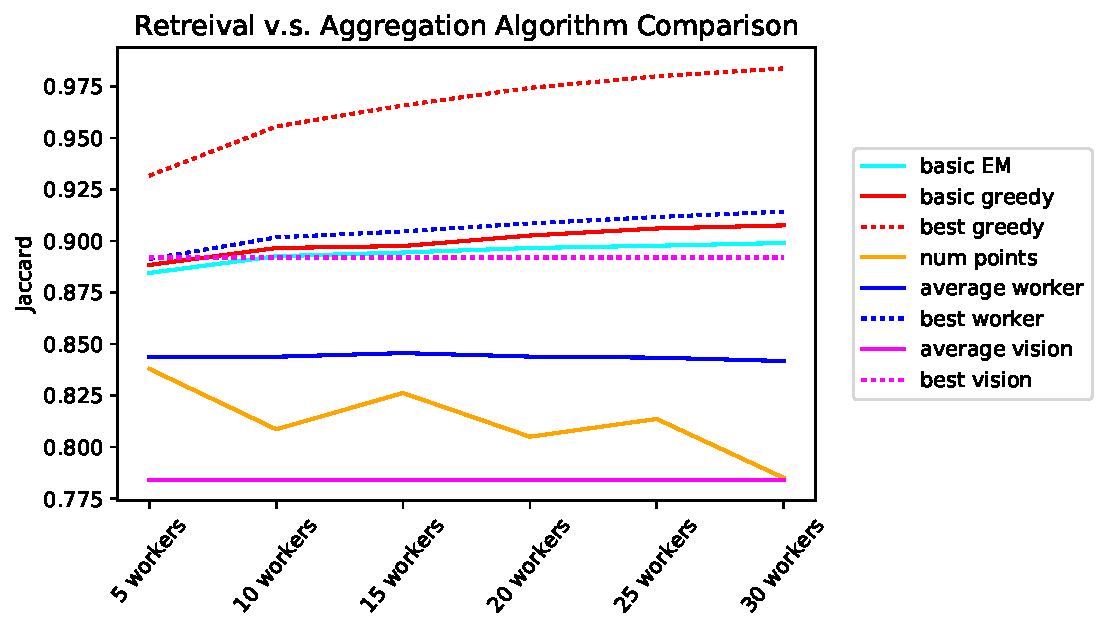
\includegraphics[width=\textwidth]{plots/Retreival_vs_Aggregation.pdf}
      \caption{Jaccard performance comparison between best-performing algorithms from retrieval and aggregation-based methods, with clustering as a preprocessing step where possible. Color denotes the type of algorithm used.}
      \label{retreival_vs_aggregation}
    \end{figure}
    \dor{We should split w/ GT and no GT information into two plots side by side with same color scheme. Also consider merging greedy and EM into just one that says aggregation based method, and renaming num points as retrevial based methods.}
    \par Table~\ref{workerScaling} shows that the three retrieval-based methods on the left do not improve the resulting Jaccard significantly when more annotations are used, whereas the right four aggregation-based methods improves significantly from the 5 worker to 30 worker sample. Intuitively, the worker scaling of retrieval-based methods is not guaranteed \footnote{except in the case of picking the best worker, the more samples means higher probability that there would be a better segmentation}. On the other hand, since larger worker samples results in finer granularity tiles for the aggregation-based methods, there is an monotonically increasing relationship between number of worker segmentation used in the sample and performance due to the finer tiles set created by multiple segmentations.
      \begin{table}
      \small
        \setlength\tabcolsep{1.5pt}
        \begin{tabular}{l|l|l|llll}
\multicolumn{3}{l|}{Retrieval-based} & \multicolumn{4}{l}{Aggregation-based}                                                             \\ \hline
num pts  & avrg worker & best worker & \multicolumn{1}{l|}{MV}   & \multicolumn{1}{l|}{EM}   & \multicolumn{1}{l|}{greedy} & best greedy \\ \hline
-6.30    & -0.25       & 2.58        & \multicolumn{1}{l|}{1.63} & \multicolumn{1}{l|}{1.64} & \multicolumn{1}{l|}{2.16}   & 5.59       
\end{tabular}
        \caption{Percentage change in Jaccard between 5 workers samples and 30 workers sample averages.}
        \label{workerScaling}
        \vspace{-10pt}
      \end{table}
      % as well as operating at a finer granularity that results in a higher potential upper bound.} 
      %Future work on developing better inference models would bring the performance closer to these upper bounds.
       \ta{Since aggregation-based methods operate at a finer tile-based granularity than whole-segmentation retrieval methods, the performance of aggregation-based approaches is better and also scales well as more annotations are collected.} 
%%%%%%%%%%%%%%%%%%%%%%%%%%%%%%%%%%%%%%%%%%%%%%%%%%%%%%%%%%%%%%%%%%%%%%%%%%%%%%%%%%%%%%%%%%%%%%%%%%%%%%%%%%%%%%%%%%%%%%%%%%%%%%%%%%%%%%%%%%
  \subsection{How well does the inferred worker qualities predict individual worker performance?}
    \subsubsection{Correlation of worker qualities against performance}
     To further investigate how the EM models are performing, we looked at whether the model-inferred worker qualities is indicative of the actual quality of a segmentation. We performed linear fitting independently for each sample-objects and computed the $R^2$ statistics to determine whether worker qualities can accurately predict precision, recall, and Jaccard scores. Visual inspection of the basic worker quality model fitting showed that for objects that suffered from type two errors (semantic ambiguity), the single-parameter worker quality was unable to capture the overbounding behavior, which lead to a low precision and Jaccard. The results are listed in Table \ref{correlation} to highlight how our advanced worker qualities were able to better capture these scenarios. The clustering preprocessing was not performed for the values in Table \ref{correlation} to demonstrate the sole effect of the EM algorithm. Nevertheless, our clustered results also show a similar trend, with an average of $R^2$=0.88 and 0.89 for the GT and GTLSA models across all objects respectively. We also find that in general the linear fit improves as the number of data points increases, which indicates consistency in the fitted model.
    \begin{table}[ht!]
    \small
      \begin{tabular}{ccccccc}
        \hline
           N &   basic &   GT &   GTLSA &   isobasic &   isoGT &   isoGTLSA \\
        \hline
              5 &      0.601 &   0.907 &      0.901 &       0.576 &    0.907 &       0.904 \\
            10 &      0.632 &   0.895 &      0.899 &       0.633 &    0.895 &       0.898 \\
            15 &      0.622 &   0.897 &      0.898 &       0.622 &    0.897 &       0.897 \\
            20 &      0.636 &   0.894 &      0.899 &       0.637 &    0.894 &       0.898 \\
            25 &      0.66  &   0.901 &      0.905 &       0.661 &    0.901 &       0.904 \\
            30 &      0.673 &   0.907 &      \cellcolor{blue!25}0.914 &       0.676 &    0.907 &       \cellcolor{blue!25}0.913 \\
        \hline
      \end{tabular}
        \caption{Linear correlation of worker qualities against ground truth performance for different quality models across different number of workers (N). The lower worker samples exhibit lower $R^2$ due to the variance from smaller number of datapoints for each independent fit. }
        \label{correlation}
    \end{table}
    \vspace{-10pt}
    % \subsubsection{EM performance with different worker quality models}
    %   - why is iso cases not performing as well
    \subsubsection{Best worker quality retrieval}
    One application of worker qualities is that it could be used as an annotation scoring function for retrieving the best quality worker segmentation. We explore this approach by training a linear regression model for every sample-object and use the worker qualities to predict the precision, recall, and Jaccard of individual worker annotations against ground truth. Then, we query the model with the inferred worker quality and retrieve the worker with the best predicted Jaccard. 
    \par The reason why a linear regression model was chosen rather than simply sorting the worker qualities and picking the best is that sorting based on multiple worker qualities (precision, recall, Jaccard) effectively applies equal weighting to all quality attributes, whereas our advanced models are specifically designed to capture cases of false-positives and false-negatives that can yield drastically different recall and precision values. We have tested that the linear regression model performs better on this task that simple sorting is capable of learning the weights that helps it make better predictions. As shown in Table~\ref{bigtable}, the performance of worker-quality based retrieval is comparable the performance other aggregation-based methods. We find that amongst the different worker quality models, advanced worker quality models perform the best, agreeing with our intuition regarding correlation results observed in Table~\ref{correlation}.
    \begin{table}[ht!]
    \small
    \setlength\tabcolsep{3pt}
    \begin{tabular}{lrrrrrr}
      \hline
       algo/N                  &     5 &    10 &    15 &    20 &    25 &    30 \\
      \hline
       num points           & 0.838 & 0.809 & 0.826 & 0.805 & 0.814 & 0.785 \\
       best worker          & 0.891 & 0.902 & 0.905 & 0.909 & 0.912 & 0.914 \\
       \hline
       MV                   & 0.885 & 0.893 & 0.894 & 0.897 & 0.898 & 0.899 \\
       EM[basic]           & 0.884 & 0.893 & 0.894 & 0.897 & 0.898 & 0.899 \\
       EM[GT]              & 0.885 & 0.893 & 0.894 & 0.897 & 0.898 & 0.899 \\
       EM[GTLSA]           & 0.871 & 0.892 & 0.891 & 0.896 & 0.897 & \cellcolor{blue!25} 0.899 \\
       greedy               & 0.888 & 0.896 & 0.896 & 0.902 & 0.905 & 0.906 \\
       wqr[basic]          & 0.878 & 0.877 & 0.877 & 0.877 & 0.878 & 0.878 \\
       wqr[GT]             & 0.884 & 0.885 & 0.885 & 0.885 & 0.887 & 0.887 \\
       wqr[GTLSA]          & 0.874 & 0.881 & 0.883 & 0.885 & 0.886 & \cellcolor{blue!25} 0.887 \\
      \hline
    \end{tabular}
    \caption{Summary of average performance across workers with clustering applied as preprocessing in all algorithms across different number of workers (N). wqr is the abbreviation for best worker quality retrieval methods.}
    \label{bigtable}
    \end{table}
%%%%%%%%%%%%%%%%%%%%%%%%%%%%%%%%%%%%%%%%%%%%%%%%%%%%%%%%%%%%%%%%%%%%%%%%%%%%%%%%%%%%%%%%%%%%%%%%%%%%%%%%%%%%%%%%%%%%%%%%%%%%%%%%%%%%%%%%%%
  \subsection{How do different families of aggregation-based algorithms relate and compare?}
  Given the success of aggregation-based models, we wanted to further study how different algorithms perform compared to one another. \ta{As shown in Table~\ref{bigtable}, majority vote, while simple, performs nearly as well as the advanced EM and greedy based approaches.} This is because both EM and greedy have learned worker qualities that converged to MV behavior\ads{need help with this explanation}.
   \par As shown in the dotted and solid line pairs in Figure~\ref{retreival_vs_aggregation}, when using ground truth to estimate intersection areas, we can achieve an average Jaccard of 0.983 as an upper bound with the 30 workers sample, which indicates that with better probabilistic estimation of intersection area, aggregation-based methods can achieve close to perfect segmentation outputs, exceeding the results than achievable by any single `best' worker (J=0.91 for 30 workers). Algorithms that gives users the option for collecting highly-accurate segmentation can have several useful applications in the biomedical domain~\cite{Gurari2015}.
%%%%%%%%%%%%%%%%%%%%%%%%%%%%%%%%%%%%%%%%%%%%%%%%%%%%%%%%%%%%%%%%%%%%%%%%%%%%%%%%%%%%%%%%%%%%%%%%%%%%%%%%%%%%%%%%%%%%%%%%%%%%%%%%%%%%%%%%%%
  \subsection{How well does clustering resolve multiple perspectives of crowdworkers and improve quality evaluation algorithms?}
    Figure \ref{cluster_example} demonstrates how spectral clustering is capable of dividing the worker responses based on pairwise mutual Jaccard into clusters with meaningful semantic associations, reflecting the crowd's diversity of perspectives in completing same task.
    \begin{figure}[ht!]
      \centering
      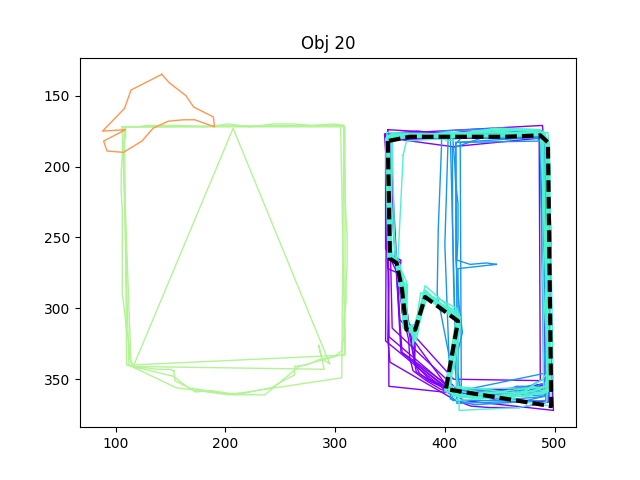
\includegraphics[width=\textwidth]{plots/20.png}
      \caption{Example image showing clustering performed on the same object from Figure \ref{error_examples}.}
      \label{cluster_example}
    \end{figure}
  \par Compared to using a metric-based heuristic to detect and eliminate these errors, clustering has additional benefit of preserving worker's semantic intentions in the case where there are multiple instances of different errors. For example, in Figure \ref{cluster_example}, the mistakened clusters included semantic concepts ``monitor'' and ``turtle''. While these are considered bad annotations for this particular task, this cluster of annotation can provide more data for another semantic segmentation task ``monitor''. A potential direction of future work includes adding a additional crowdsourcing task for semantic labelling of clusters (which is cheaper and more accurate than segmentation) to enable reuse of annotations across objects and lower the cost of data collection. 
  \par In addition to perspective resolution, clustering results can also be used as a preprocessing step to any of the quality evaluation algorithms that we have discussed. The clustering preprocessing can significantly improve algorithms that are not very robust to segmentations that contain semantic errors or regional semantic ambiguity issues, such as the heuristic-based number of points approach. When examining the gap of increase with and without clustering in Figure \ref{cluster_effect}, we find that aggregation-based methods performs better than retrieval-methods exhibits a smaller gap between the performances. This effect is due to aggregation-based method's higher performance in the no cluster case, indicating that it is able to capture some of the semantic ambiguity and errors in the dataset.
    \begin{figure}[ht!]
      \centering
      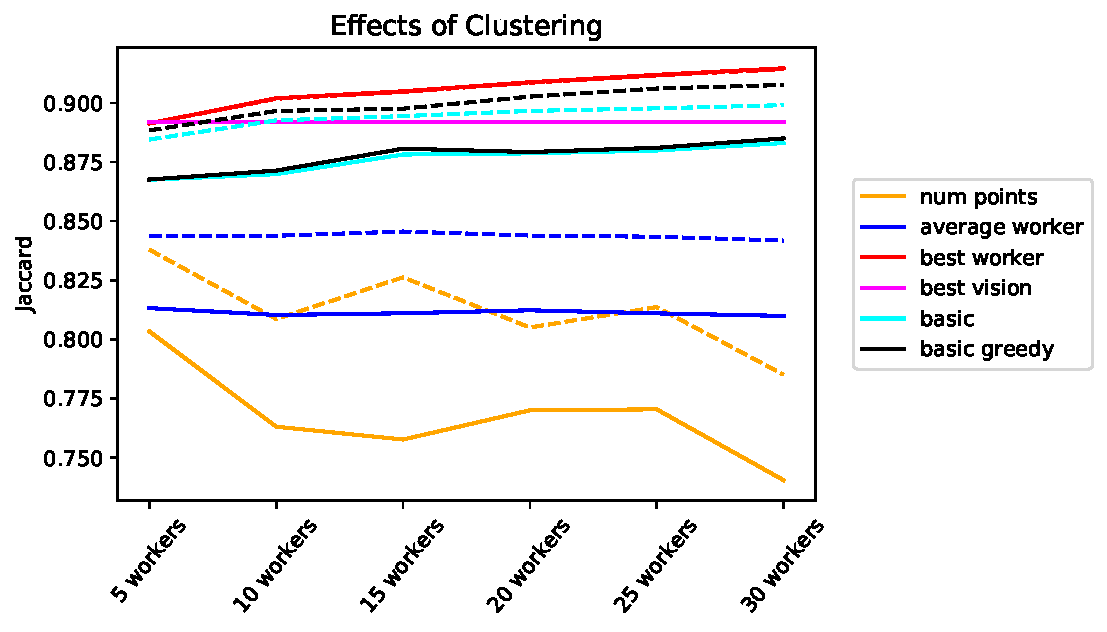
\includegraphics[width=\textwidth]{plots/Effects_of_clustering.pdf}
      \caption{Performance comparisons between averaging over experiments with clustering as a preprocessing step(dotted) and the unclustered cases(solid) for different algorithms.}
      \label{cluster_effect}
    \end{figure}
  %if time permits add table with stats showing how much increase in performance.
% %%%%%%%%%%%%%%%%%%%%%%%%%%%%%%%%%%%%%%%%%%%%%%%%%%%%%%%%%%%%%%%%%%%%%%%%%%%%%%%%%%%%%%%%%%%%%%%%%%%%%%%%%%%%%%%%%%%%%%%%%%%%%%%%%%%%%%%%%%
%   \subsection{Can vision information be used to improve the crowdsourced responses?}
%   We explored the idea of using a vision algorithm to improve aggregation-based quality evaluation methods. 